\documentclass[12pt,reqno,a4paper,oneside]{article}

\usepackage{amsfonts, amsmath,
	        amssymb, amsthm}  % Fontes e símbolos matemáticos da AMS.
\usepackage{graphicx}         % Importação de gráficos.
\usepackage{subfig}
\usepackage[brazil]{babel}    % Idioma português (Brasil) como padrão.
\usepackage[utf8]{inputenc}   % Codificação UTF-8.
%\usepackage{natbib}           % Para citações.
%\usepackage{cite}             % Idem.

\usepackage{bm}          % Equações em negrito com qualidade superior.
\usepackage{booktabs}    % Edição de linhas de tabelas.
\usepackage{caption}     % Edição do texto dos títulos de tabelas.
\usepackage{color}       % Edição de cores.
\usepackage{indentfirst} % Indentará sempre o 1º parágrafo de cada seção do relatório.
%\usepackage{enumitem}   % Edição mais elaborada de listas
                         % Conflito com ambiente "enumerate" no beamer!.
%\usepackage{hyperref}   % Criação de "hyperlinks".
\usepackage{multirow}    % Para obter uma célula com uma coluna e várias linhas.
\usepackage{ragged2e}    % Opções de alinhamento do texto.

%\usepackage[FIGTOPCAP]{subfigure} % Acesso a figuras dentro de pastas.

\usepackage[top=2cm, bottom=2cm,
            left=2cm, right=2cm]{geometry} % Margens do texto.

\captionsetup{justification = centering} % Centraliza os títulos das tabelas.

% Símbolo matemático para independência entre variáveis aleatórias:

\newcommand\indep{\protect\mathpalette{\protect\independenT}{\perp}}\def\independenT#1#2{\mathrel{\rlap{$#1#2$}\mkern2mu{#1#2}}}

\begin{document}

\title{\huge Relatório do Trabalho de\\
	Estatística Bayesiana I}
\author{\\
	\\
	\huge Mistura de Normais\\
	\huge com Variância Contaminada\\
	\\
	\\
	\\
	\\
	\Large Caio Balieiro\\
	\Large Taiguara Melo Tupinambás\\
	\Large Walmir dos Reis Miranda Filho\\
	\\
	\\
	\\
	\\
	\Large Prof. Dani Gamerman\\
	\Large Profª Rosangela Helena Loschi\\
	\\
	\\
	\\
	\\
	\\
	Programa de Pós-Graduação em Estatística\\
	Instituto de Ciências Exatas\\
	Universidade Federal de Minas Gerais\\
	\\
	\\
	\\
	\\
	\\
	\\}
\date{Belo Horizonte, 2 de dezembro de 2019}
\maketitle

\newpage

\section{\Large Introdução}

O presente trabalho tem como objetivo obter, dada uma densidade \textit{a posteriori} conjunta dos parâmetros de um modelo probabilístico para uma amostra previamente observada, as densidades marginais de cada parâmetro, bem como as estatísticas de média; variância; assimetria e curtose associadas, a partir da implementação de três métodos numéricos, a saber: (i) integração via quadratura de Riemann; (ii) reamostragem por importância sequencial (em inglês, \textit{Sequential Importance Resampling}, ou SIR); e (iii) integração via Monte Carlo em cadeias de Markov (em inglês, \textit{Markov chain Monte Carlo}, ou MCMC) com inovações dadas pelo algoritmo de Metropolis-Hastings (MH).

Para o modelo que gerou a amostra observada, será pressuposto que sua especificação é dada por uma mistura finita de normais. Sejam $X_{1}, \ldots, X_{n}$ amostras aleatórias independentes, condicionalmente a um vetor de parâmetros $\bm{\theta} = (\mu, \sigma^2, \nu)$, e identicamente distribuídas com função densidade dada por
\begin{equation}\label{eq:dist_am}
f(x | \mu, \sigma^2, \nu) = \nu \phi(x | \mu, 100 \sigma^2) + (1 - \nu) \phi(x | \mu, \sigma^2), \ x \in \mathbb{R},
\end{equation}
\noindent onde $\phi(x | \mu, \sigma^2) = (2\pi\sigma^2)^{-1} \exp[-(x - \mu)^2/(2\sigma^2)]$ denota a função densidade da distribuição normal com média $\mu$ e variância $\sigma^2$ avaliada no ponto $x$. Para o suporte de cada parâmetro, tem-se que $\mu \in \mathbb{R}, \sigma^2 \in \mathbb{R}_+$ e $\nu \in (0,1)$.

A mistura finita descrita em \eqref{eq:dist_am} possui duas componentes normais que diferem nas respectivas variâncias: para a primeira componente, o valor é 100 vezes o da segunda. Desta forma, tem-se uma mistura finita de normais com variância \textit{contaminada}.

Para os parâmetros $\mu$, $\sigma^2$ e $\nu$, será pressuposto que cada um segue uma distribuição \textit{a priori} predeterminada: $\mu | \sigma^2 \sim{N} (m, V \sigma^2)$, onde $N(\cdot)$ denota a distribuição normal com média $m \in \mathbb{R}$ e variância $V \sigma^2$, $V > 0$; $\sigma^2 \sim{GI} (a,d)$, onde $GI(\cdot)$ denota a distribuição gama inversa com parâmetros de forma $a > 0$ e de taxa $d > 0$ (inverso da escala); e $\nu \sim{U}(0,1)$, a distribuição uniforme contínua padrão.

Para gerar uma amostra aleatória do modelo em $\eqref{eq:dist_am}$, foi utilizada uma representação hierárquica (Lachos \textit{et al.}, 2013)\cite{Lachos2013} tal que
\begin{equation}
X_i | \mu, \sigma^2, U_{i} = u_i \sim{N}(\mu, \sigma^2 u_i^{-1}), \quad U_i | \mu \sim{p_d}(1,100) : P(U_i = 100) = \nu. \label{eq:hier}
\end{equation}
\noindent onde $p_d(a,b)$ denota uma função de probabilidade (discreta) que atribui massa probabilística apenas aos pontos $a$ e $b$.

A partir do produto entre a função de verossimilhança $f(\bm{x} | \mu, \sigma^2, \nu)$ para uma amostra $\bm{x} = (x_1, \ldots, x_n)$ gerada através da representação hierárquica em \eqref{eq:hier} e das densidades \textit{a priori} para cada parâmetro do modelo, obtém-se o núcleo (em inglês, \textit{kernel}) da densidade \textit{a posteriori} conjunta $p(\mu, \sigma^2, \nu | \bm{x})$. Como a expressão da densidade \textit{a posteriori} possui uma constante de proporcionalidade $f(x_1, \ldots, x_n) = f(\bm{x})$ não facilmente calculável, mas que não depende dos parâmetros, pode-se usar o núcleo daquela para inferir sobre cada um dos parâmetros. No modelo de mistura finita de duas componentes normais com variância contaminada, temos que
\begin{align}
p(\mu, \sigma^2, \nu | \bm{x})
&= \dfrac{f(\bm{x} | \mu, \sigma^2, \nu) \times p(\mu, \sigma^2, \nu)}{f(\bm{x})} \propto \prod_{i=1}^{n} f(x_i) \times p(\mu | \sigma^2) \times p(\sigma^2) \times p(\nu) \nonumber\\
&\propto \prod_{i=1}^{n} \left[ \nu \phi(x_i | \mu, 100 \sigma^2) + (1 - \nu) \phi(x_i | \mu, \sigma^2) \right] \times \nonumber \\
&\times \phi(\mu | m, V \sigma^2) \times \dfrac{d^a}{\Gamma(a)} \left(\dfrac{1}{\sigma^2}\right)^{a + 1} \exp\left(-\dfrac{d}{\sigma^2}\right) \nonumber \\
&\propto \left(\dfrac{1}{\sigma^2}\right)^{(n + 1)/2 + a + 1} \exp\left\{-\dfrac{\left[(\mu - m)^2 / (2V) + d\right]}{\sigma^2}\right\} \times \textrm{A}(\bm{x} | \mu, \sigma^2, \nu), \label{eq:dist_post}
\end{align}
onde
\begin{equation*}
\textrm{A}(\bm{x} | \mu, \sigma^2, \nu) = \prod_{i=1}^{n} \left\{  \dfrac{\nu}{10} \exp\left[-\dfrac{(x_i - \mu)^2}{200\sigma^2}\right] + (1 - \nu) \exp\left[-\dfrac{(x_i - \mu)^2}{2\sigma^2}\right] \right\}
\end{equation*}

Evidentemente, trabalhar diretamente com o lado direito em \eqref{eq:dist_post} não é computacionalmente agradável, uma vez que esta é um produto de várias quantidades sempre menores do que 1, muitas delas próximas de 0, o que pode levar a problemas de aproximação numérica. Desta forma, sempre que for necessário calcular o núcleo da \textit{posteriori}, dada uma amostra, inicialmente será tomada a soma do logaritmo de todos as quantidades que compõem este produto e só depois esta mesma soma será exponenciada. Dependendo do quão negativa for a soma (o logaritmo de termos entre 0 e 1 é sempre negativo), quando exponenciada ela pode ou não ser numericamente igual a 0.

Logo, na geração da amostra $\bm{x}$ deve-se escolher valores de $\mu$, $\sigma^2$ e $\nu$ tais que o núcleo de $p(\mu, \sigma^2, \nu | \bm{x})$ não seja numericamente nulo para os verdadeiros valores dos parâmetros. Considerando o uso da linguagem de programação \textit{R} (R Core Team, 2019)\cite{RCoreTeam2019}, esta escolha não é difícil. Na versão 3.5.3, o menor valor que pode ser tomado como argumento da função \verb|exp()| do \textit{R} é $-709$. Desta forma, basta tomar $\mu$, $\sigma^2$ e $\nu$ tais que o logaritmo do lado direito em \eqref{eq:dist_post} seja maior do que $-709$.

Para o presente trabalho, foram considerados uma amostra de tamanho $n=500$ (Figura \ref{fig:sample_n}) da mistura finita de normais com variância contaminada parametrizada de tal forma que $\mu = 11$; $\sigma^2 = 0.64$ e $\nu = 0.2$, com hiperparâmetros $m = 11$; $V = 1$; $a = 7$ e $d = 4$ nas distribuições \textit{a priori}. Fixada uma semente aleatória, para a amostra gerada a partir dos valores citados, o logaritmo do núcleo da densidade \textit{a posteriori} foi igual a $-518.9061$, cuja exponencial é aproximadamente igual a $4.385 \times 10^{-226}$.

\begin{figure}[htb]
	\centering
	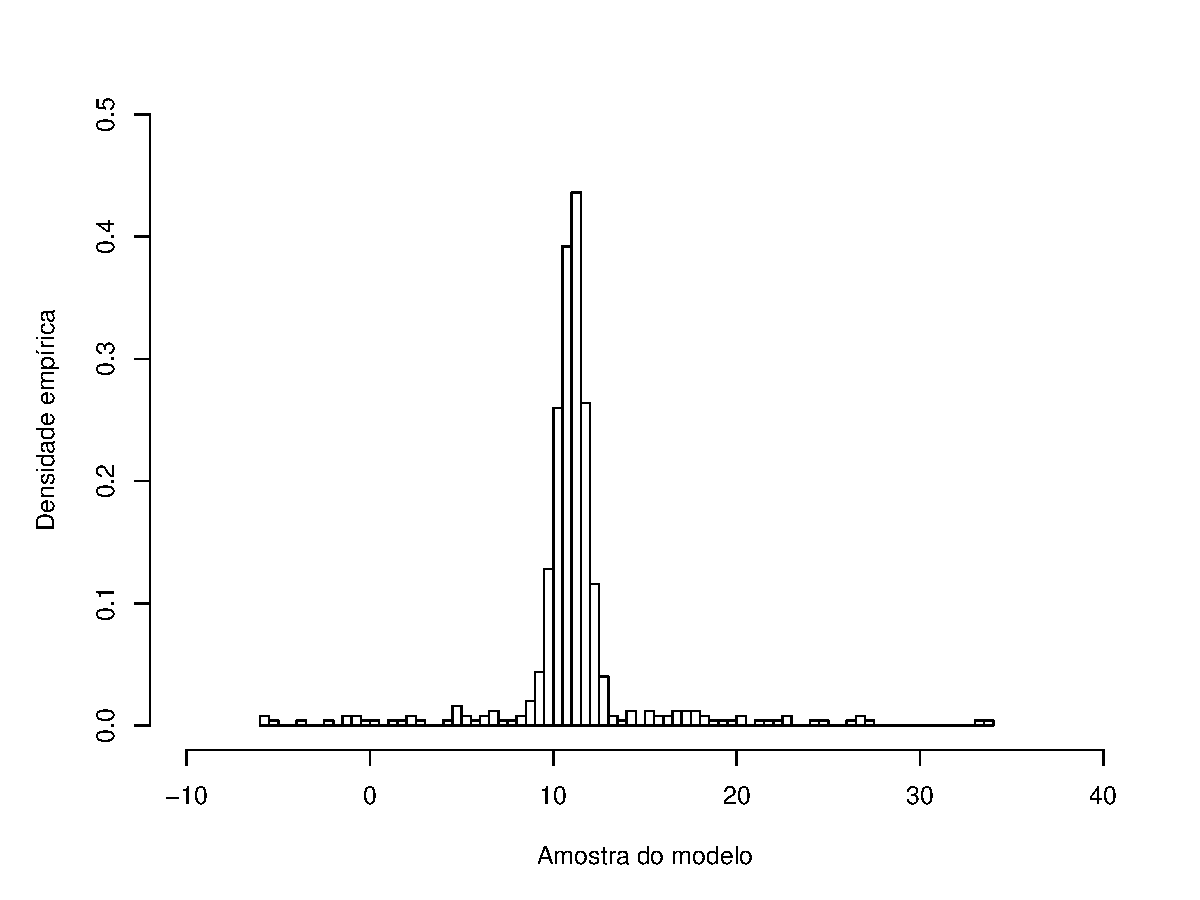
\includegraphics[scale=0.8]{figuras/amostra_n.pdf}
	\caption{Histograma da amostra gerada do modelo}
	\label{fig:sample_n}
\end{figure}

Como não se tem uma expressão fechada para $p(\mu, \sigma^2, \nu | \bm{x})$, mas apenas de seu núcleo, para obter as densidades marginais de $\mu$, $\sigma^2$ e $\nu$ dado $\bm{x}$, bem como as estatísticas associadas a cada uma delas, é necessário aproximá-las por algum método numérico. Na seções \ref{quarie}, é apresentado o primeiro dos três métodos considerados: a integração via quadratura de Riemann. Por sua vez, na seção \ref{sir} é descrito o método SIR. Por fim, na seção \ref{mcmc}, é retratada a integração via MCMC com inovações MH. Todos os métodos serão testados e comparados no contexto do modelo exposto acima. Na seção \ref{consfin}, são resumidos os resultados obtidos para os três métodos, bem como é feita uma avaliação comparativa da qualidade de sua convergência.

Antes de implementar cada um dos métodos numéricos, foram feitos três gráficos (Figuras \ref{fig:maspro_mu} a \ref{fig:maspro_nu}) do núcleo de $p(\mu, \sigma^2, \nu | \bm{x})$ quando se varia um dos três parâmetros e os outros dois são mantidos fixos nos respectivos valores verdadeiros pressupostos para o modelo que gerou a amostra. Tais gráficos permitem dizer, para cada parâmetro, quais são os intervalos do suporte correspondente que concentram praticamente toda a massa probabilística da densidade marginal \textit{a posteriori} associada, ainda que as densidades calculadas sejam válidas apenas quando os outros dois parâmetros são fixados em valores arbitrários. Esta informação será útil para definir os intervalos de integração na quadratura de Riemann e a matriz de covariância da distribuição proposta nos métodos SIR e MCMC-MH para aproximação das densidades marginais verdadeiras.

\begin{figure}[htb]%
	\centering
	\subfloat[Intervalo para $\mu$ dados $\sigma^2 = 0.64, \nu = 0.2$]{
		{
			\label{fig:maspro_mu}
			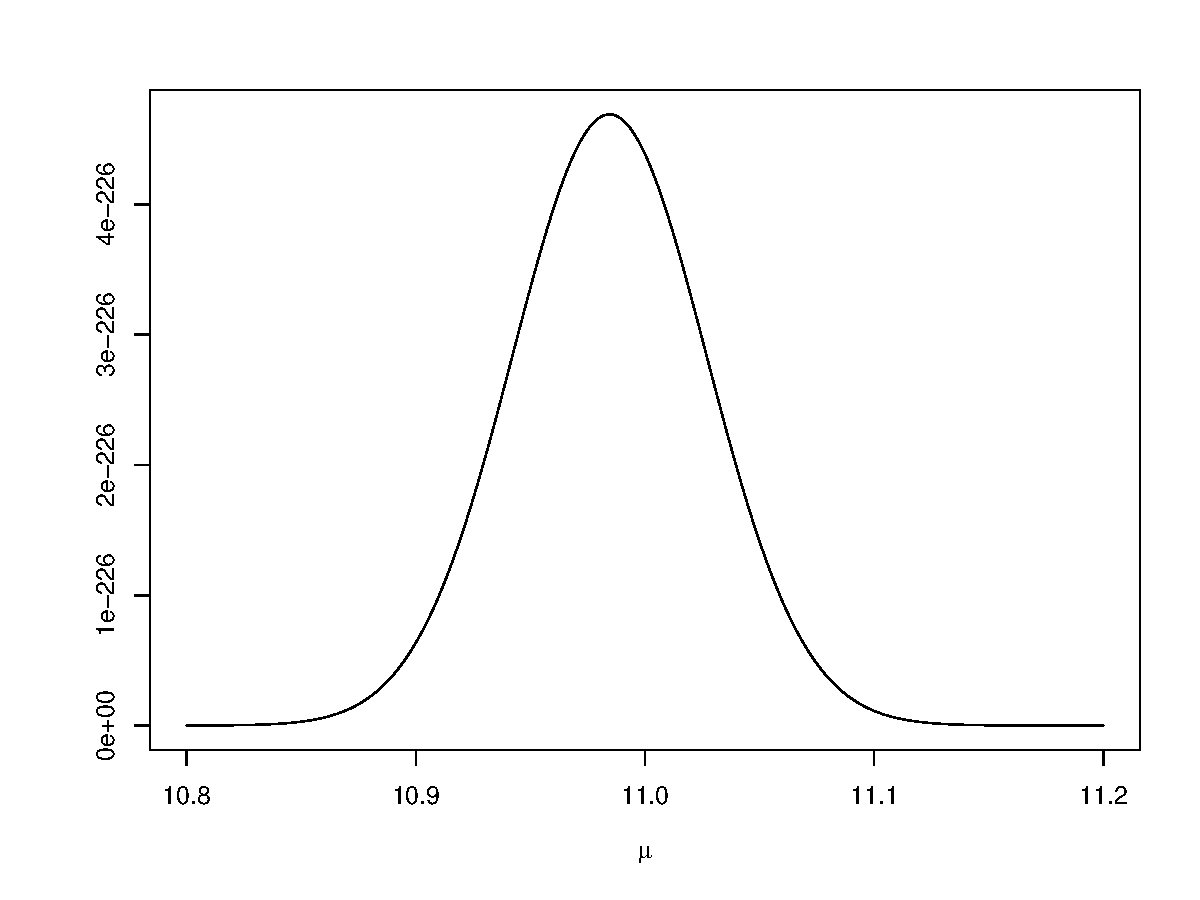
\includegraphics[scale=0.4]{figuras/maspro_mu.pdf}}}%
	\qquad
	\subfloat[Intervalo para $\sigma^2$ dados $\mu = 11, \nu = 0.2$]{
		{
			\label{fig:maspro_s2}
			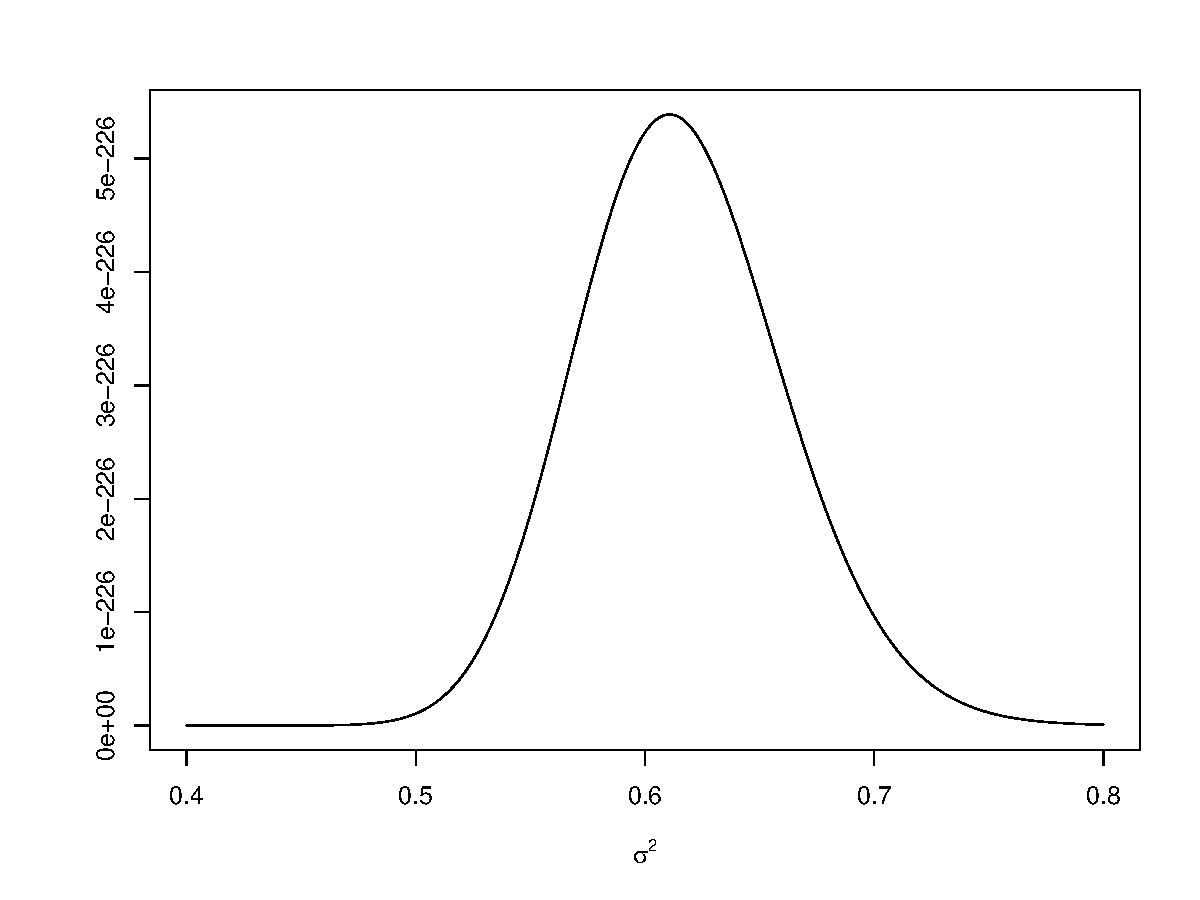
\includegraphics[scale=0.4]{figuras/maspro_s2.pdf}}}%
	\subfloat[Intervalo para $nu$ dados $\mu = 11, \sigma^2 = 0.64$]{
		{
			\label{fig:maspro_nu}
			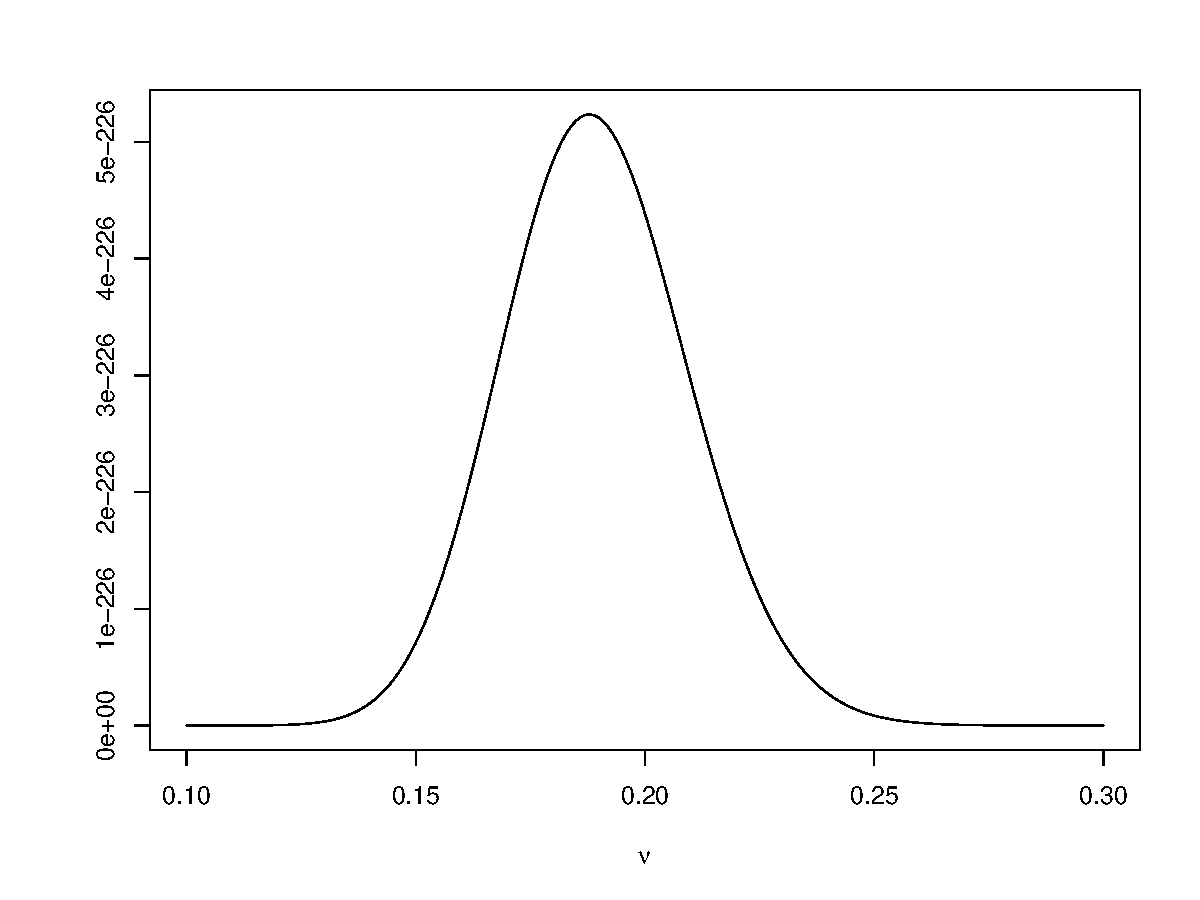
\includegraphics[scale=0.4]{figuras/maspro_nu.pdf}}}%
	\caption{Intervalos de massa probabilística para cada parâmetro (variável aleatória) do núcleo de $p(\mu, \sigma^2, \nu | \bm{x})$}%
\end{figure}

\section{\Large O Método da Quadratura de Riemann}\label{quarie}

%Texto descrevendo o método e como foi feita neste trabalho a aproximação via quadratura de Riemann.

\section{\Large O Método da Reamostragem Ponderada}\label{sir}

%Texto descrevendo o método e como foi feita neste trabalho a geração de variáveis aleatórias da distribuição de interesse usando este mesmo método.

\section{\Large O Método de Monte Carlo via Cadeias de Markov}\label{mcmc}

%Texto descrevendo o método e como foi feita neste trabalho a geração de variáveis aleatórias da distribuição de interesse usando este mesmo método, bem como o amostrador selecionado (possivelmente Gibbs ou outro que for de melhor uso para todo o grupo).

\section{Considerações Finais}\label{consfin}

%Texto descrevendo de forma resumida o que foi feito nas seções anteriores, bem como os resultados dos métodos quanto à convergência, à medida que se aumenta o tamanho amostral m da distribuição \textit{a poseteriori}.

\bibliographystyle{unsrt}
\bibliography{ref}

\end{document}